
%%%%%%%%%%%%%%%%%%%%%%%%%%%%%%%%%%%%%%%%%%%% Articolo - A4 - Landscape


%%%%%%%%%%%%%%%%%%%%%%%%%%%%%%%%%%%%%%%%%%%% preambolo

\documentclass[11pt, landscape]{article}
\usepackage[utf8]{inputenc}
\usepackage[italian]{babel}
\usepackage{multicol}
\usepackage{caption}
\captionsetup{justification   = raggedright,
              singlelinecheck = false}
\setlength{\columnsep}{1cm}
\usepackage[margin=1in]{geometry}
\usepackage{amsfonts, amsmath, amssymb}
\usepackage[none]{hyphenat}
\usepackage{fancyhdr}
\usepackage{graphics}
\usepackage{float}
\usepackage[nottoc, notlot, notlof]{tocbibind}
\usepackage{pgf,tikz,pgfplots} 
\pgfplotsset{compat=1.15}
\usepackage{mathrsfs}
\usetikzlibrary{arrows}

\pagestyle{fancy}
\fancyhead{}
\fancyfoot{}
\fancyhead[L]{\small \MakeUppercase{lezioni di matematica per il Liceo}}
\fancyhead[R]{\small \emph{prof. Diego Fantinelli}}
\fancyfoot[C]{\thepage}
\renewcommand{\headrulewidth}{0.5pt}
\renewcommand{\footrulewidth}{0.1pt}

\parindent 0ex
\setlength{\parindent}{4em}
\setlength{\parskip}{1em}
\renewcommand{\baselinestretch}{1.5}

%%%%%%%%%%%%%%%%%%%%%%%%%%%%%%%%%%%%%%%%%%%% title page

\begin{document}

\begin{titlepage}
\begin{center}
\vspace*{1cm}
\Large{\textbf{Matematica - Lezioni per il Liceo}}\\
\large{\textbf{- Sottotitolo -}}\\
\vfill
\line(1,0){400}\\[.5mm]
\huge{\textbf{TITOLO ARGOMENTO}}\\[3mm]
\Large{\textbf{- Sottotitolo: prova ipad -}}\\[1mm]
\line(1,0){400}\\
\vfill
{\scriptsize By Student Name}\\
{\scriptsize Candidate \#} \\
{\scriptsize \today} \\

\end{center}
\end{titlepage}

%%%%%%%%%%%%%%%%%%%%%%%%%%%%%%%%%%%%%%%%%%%% introduzione

\tableofcontents
\thispagestyle{empty}
\clearpage

\setcounter{page}{1}

\vspace*{1cm}
\section{Introduzione}
Il presente documento contiene le principali soluzioni per la formattazione di un testo scientifico, con particolare riferimento ai testi matematici, comprensivi di \emph{formule}, e caratteri speciali

\subsection{Come recuperare l'autostima}
Sed fringilla, neque sit amet maximus luctus, neque eros fermentum ipsum, nec hendrerit leo urna id urna. Pellentesque vel odio lobortis diam placerat porttitor non auctor leo.\\

\begin{multicols}{2}

\subsection{Formule in testo \emph{multicolonne}}
Orci varius natoque penatibus et magnis dis parturient montes, nascetur ridiculus mus. Integer pretium bibendum dolor eget interdum.\\
Sed ultrices mi a lacus vestibulum aliquet. Nam tincidunt dui in pellentesque hendrerit. Phasellus diam libero, laoreet eu varius sed, vulputate a orci. Etiam odio tortor, sagittis nec quam quis, iaculis ultrices purus. Nunc semper purus nec elit mattis.\\[3mm]
$\displaystyle{\lim \limits_{x \to \infty} \frac{f(b)-f(a)}{x-a}=f'(a)}$\\[3mm]
Sed ultrices mi a lacus vestibulum aliquet. Nam tincidunt dui in pellentesque hendrerit. Phasellus diam libero, laoreet eu varius sed, vulputate a orci. Etiam odio tortor, sagittis nec quam quis, iaculis ultrices purus. Nunc semper purus nec elit mattis.\\
\begin{equation}
	\displaystyle{\int_a^b{f(x) \,dx=\lim \limits_{x \to \infty} \sum \limits_{k=1}^{n}f(x_k) \cdot \Delta x}}
\end{equation}\\
Sed ultrices mi a lacus vestibulum aliquet. Nam tincidunt dui in pellentesque hendrerit. Phasellus diam libero, laoreet eu varius sed, vulputate a orci. Etiam odio tortor, sagittis nec quam quis, iaculis ultrices purus. Nunc semper purus nec elit mattis.\\[1.5mm]
\end{multicols}

%%%%%%%%%%%%%%%%%%%%%%%%%%%%%%%%%%%%%%%%%%%% sez. 2

\section{Sezione 2}

\subsection{Come inserire le formule matematiche}
Lorem ipsum dolor sit amet, consectetur adipiscing elit. Sed varius lacus eget magna elementum, quis ultricies justo vestibulum. Proin sed dolor vel est rhoncus tristique iaculis auctor mauris.\\[3mm]
$f(x)=(x-3)^2+ \displaystyle \frac{x}{2}$ ha dominio $\mathrm{D}_f:(-\infty,+\infty)$
e range $\mathrm{R}_f:\left[\frac{1}{2},\infty\right)$.\\

\subsection{Come inserire le formule matematiche}
Lorem ipsum dolor sit amet, consectetur adipiscing elit. Sed varius lacus eget magna elementum, quis ultricies justo vestibulum. Proin sed dolor vel est rhoncus tristique iaculis auctor mauris.\\[3mm]
$f(x)=(x-3)^2+ \displaystyle \frac{x}{2}$ ha dominio $\mathrm{D}_f:(-\infty,+\infty)$
e range $\mathrm{R}_f:\left[\frac{1}{2},\infty\right)$.\\

%%%%%%%%%%%%%%%%%%%%%%%%%%%%%%%%%%%%%%%%%%%% sez. 3

\section{Sezione 3}

\subsection{Come inserire le formule matematiche}
Lorem ipsum dolor sit amet, consectetur adipiscing elit. Sed varius lacus eget magna elementum, quis ultricies justo vestibulum. Proin sed dolor vel est rhoncus tristique iaculis auctor mauris.\\[3mm]
$f(x)=(x-3)^2+ \displaystyle \frac{x}{2}$ ha dominio $\mathrm{D}_f:(-\infty,+\infty)$
e range $\mathrm{R}_f:\left[\frac{1}{2},\infty\right)$.\\

$\displaystyle{\lim \limits_{x \to \infty} \frac{f(b)-f(a)}{x-a}=f'(a)}$\\[1cm]

%%%%%%%%%%%%%%%%%%%%%% Utilizzando equation %%%%%%%%%%%%%%%%%%%%%%%%%
\begin{equation}
	\displaystyle{\lim \limits_{x \to \infty} \frac{f(b)-f(a)}{x-a}=f'(a)}
\end{equation}\\[1cm]
\emph{integrali}
\begin{equation}
	\displaystyle{\int \limits_{a}^{b}x^2 \,dx=\left[\frac{x^3}{3}\right]_{a}^{b}=\frac{b^3}{3}-\frac{a^3}{3}}
\end{equation}\\[1cm]
\emph{Sommatorie}
\begin{equation}
	\displaystyle{\sum \limits_{n=1}^{\infty}ar^n=a+ar+ar^2+\cdots+ar^n}
\end{equation}\\[1cm]
\emph{Mix}
\begin{equation}
	\displaystyle{\int_a^b{f(x) \,dx=\lim \limits_{x \to \infty} \sum \limits_{k=1}^{n}f(x_k) \cdot \Delta x}}
\end{equation}\\[1cm]
\emph{Vettori}
\begin{equation}
	\displaystyle{\vec{v}=v_1 \vec{i}+v_2 \vec{j}=\langle v_1, v_2 \rangle}
\end{equation}\\[1cm]

%\subsection{}

%%%%%%%%%%%%%%%%%%%%%% Tabelle %%%%%%%%%%%%%%%%%%%%%%%%%

\section{Capitolo 2}
\begin{figure}[h!]

%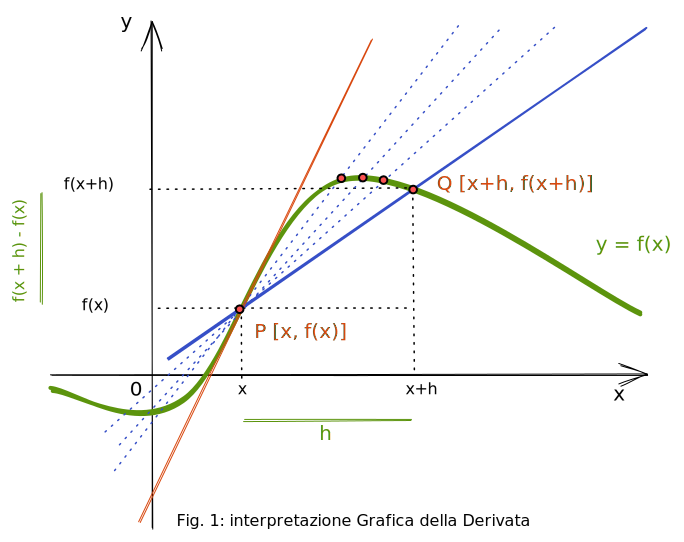
\includegraphics[width=0.5\textwidth]{Derivata}
\caption{Example of a parametric plot ($\sin (x), \cos(x), x$)}
\end{figure}
\noindent
Nam tincidunt dui in pellentesque hendrerit. Phasellus diam libero, laoreet eu varius sed, vulputate a orci. Etiam odio tortor, sagittis nec quam quis, iaculis ultrices purus. Nunc semper purus nec elit mattis.\\



	\subsection{Tabelle e Arrays}
	\begin{table}[H]
	\centering
	\caption{Relazione tra $f$ e $f'$.}
	\def\arraystretch{1.5}
	\begin{tabular}{|c|c|} % con |c| si definiscono le colonne e poi si separano le righe tra loro con \hline
	\hline
	$f(x)$ & $f'(x)$\\ \hline
	$x>0$ & La funzione $f(x)$ è \emph{crescente}. \\
	\hline
	$x<0$ & La funzione $f(x)$ è \emph{decrescente}. \\
	\hline		
	\end{tabular}
		
	\end{table}
\section{Conclusioni}

\end{document}
